\section{Ziele}
\label{sec:Ziele}
\section{Theoretische Grundlagen}
\label{sec:Theorie}
Das Geiger-Müller-Zählrohr ist ein Messinstrument um die Intensität ionisierender Strahlung zu messen.
Bei einer Absorption eines $\alpha , \beta$ oder $\gamma$ Teilchens wird vom Zählrohr ein Impuls abgegeben und es lässt sich anhand der Impulse auf die Anzahl der Teilchen schließen.
\subsection{Aufbau und Funktionsweise}
Das Geiger Müller besteht aus einem Metallzylinder als Kathode (mit Radius $r_{\text{k}}$) und einem dünnen Metalldraht in der Mitte der als Anode (mit Radius $r_{\text{a}}$).
Innerhalb des Zylinders ist ein Gasgemisch aus einem Gas und einem Alkohol Anteil (siehe: \ref{sec:Nachentladung}) das von den eintreffenden Teilchen ionisiert werden kann.
Außen an die Anode und Kathode wird eine Spannung angelegt und ein Wiederstand geschaltet.
Durch die angelegte Spannung entsteht im Zählrohrvolumen ein Radialsymmetrisches E-Feld.
\begin{equation}
    E(r) = \frac{U}{r \ln\left(\frac{r_{\text{k}}}{r_{\text{a}}}\right)}
\end{equation}
\begin{figure}
    \centering
    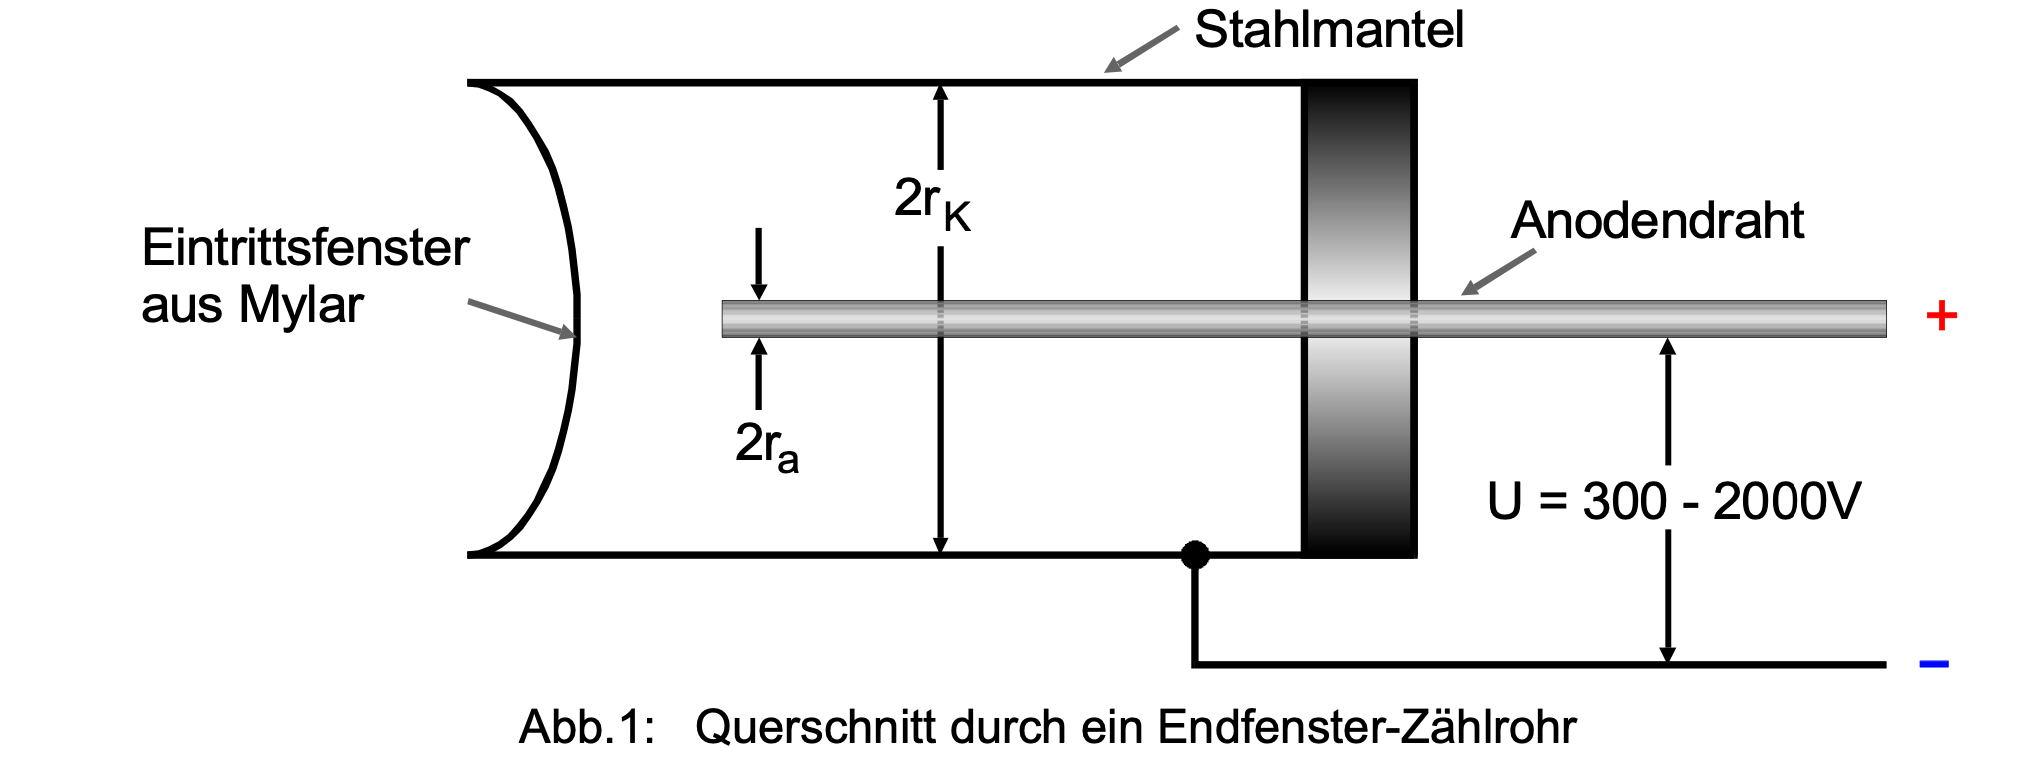
\includegraphics[width=0.3\textwidth]{bilder/Zaehlrohr_Querschnitt.png}
    \caption{Ein Zaehlrohr-Querschnitt. (Quelle \cite{Anleitung})}
    \label{fig:Zaehlrohr}
\end{figure}
Die Messung der einfallenden Teilchen und somit der Intensität ist stark abhängig von der angelegten Spannung.
\begin{figure}
    \centering
    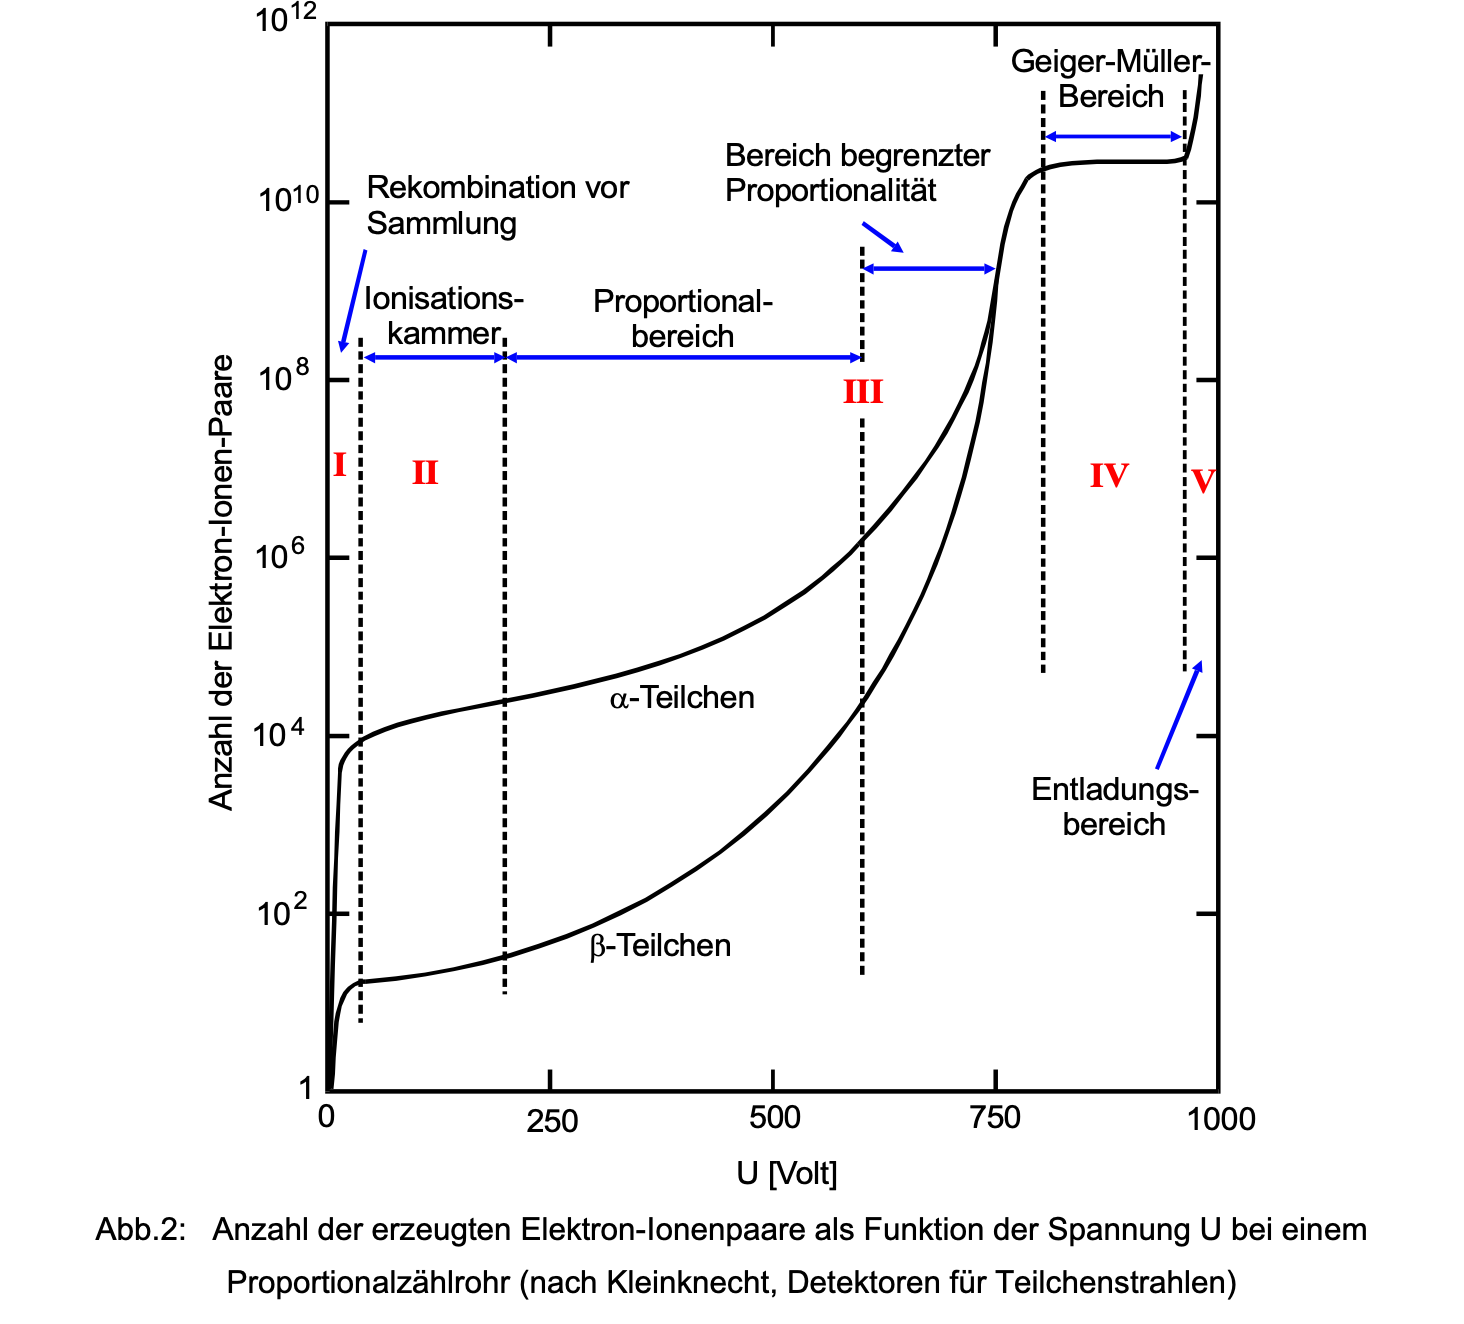
\includegraphics[width=0.5\textwidth]{bilder/Anzahl_der_Elektronen.png}
    \caption{ Anzahl der Elektronen-Ion-Paare. (Quelle \cite{Anleitung})}
    \label{fig:Anzahl_der_Elektronen}
\end{figure}
Wenn zu Beginn nur eine Sehr schwache Spannung angelegt ist reicht diese nicht aus um die Elektron Ion Paare zu trennen und sie Rekombinieren direkt wieder.
\begin{figure}
    \centering
    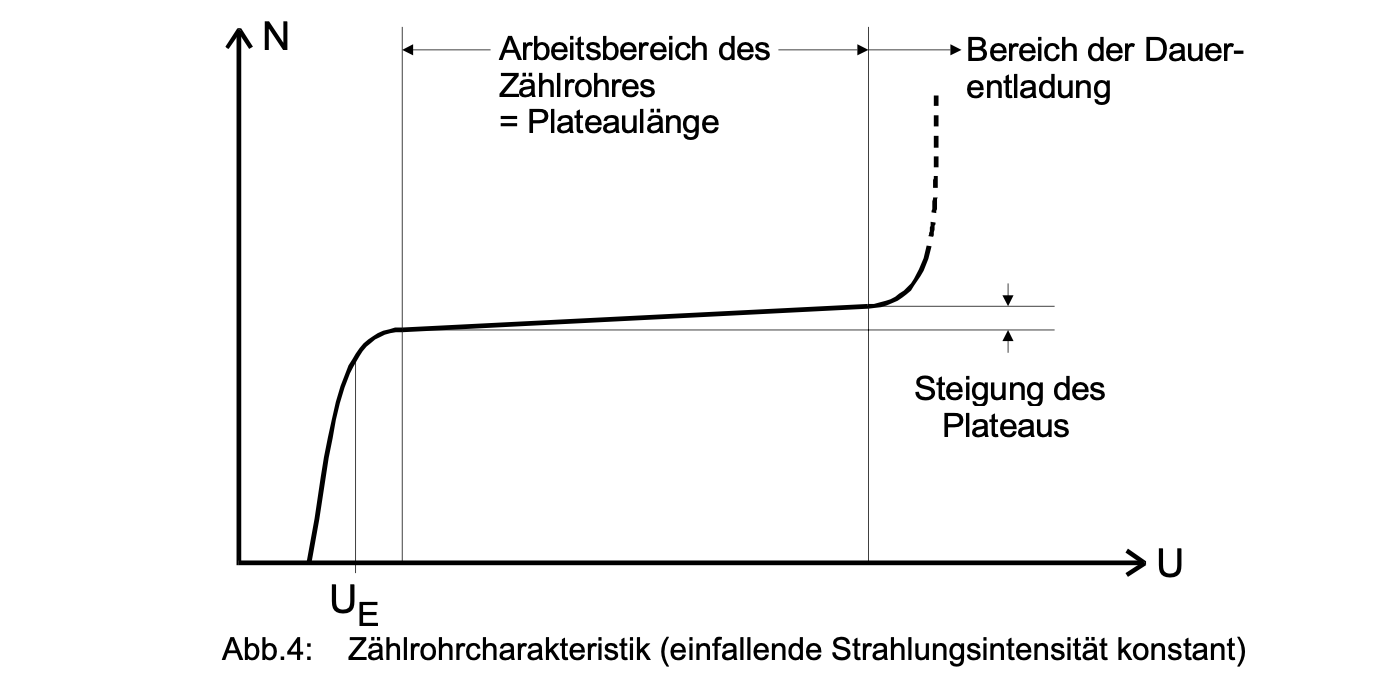
\includegraphics[width=0.5\textwidth]{bilder/Zaehlrohr_N_U_Graph.png}
    \caption{Ein N-U-Graph. (Quelle \cite{Anleitung})}
    \label{fig:Zaehlrohr_N_U_Graph}
\end{figure}
\subsubsection{Totzeit}
\subsubsection{Nachentladung}
\label{sec:Nachentladung}
\subsection{Charakteristik Geiger-Müller-Zählrohr}
